% $Header: /Users/joseph/Documents/LaTeX/beamer/solutions/conference-talks/conference-ornate-20min.en.tex,v 90e850259b8b 2007/01/28 20:48:30 tantau $

\documentclass{beamer}

% This file is a solution template for:

% - Talk at a conference/colloquium.
% - Talk length is about 20min.
% - Style is ornate.



% Copyright 2004 by Till Tantau <tantau@users.sourceforge.net>.
%
% In principle, this file can be redistributed and/or modified under
% the terms of the GNU Public License, version 2.
%
% However, this file is supposed to be a template to be modified
% for your own needs. For this reason, if you use this file as a
% template and not specifically distribute it as part of a another
% package/program, I grant the extra permission to freely copy and
% modify this file as you see fit and even to delete this copyright
% notice. 


\mode<presentation>
{
  \usetheme{Warsaw}
  % or ...
 % \setbeamercovered{transparent}
  % or whatever (possibly just delete it)
}

\usepackage[slantfont,boldfont]{xeCJK}
\setCJKmainfont{STKaiti}   % STFangsong 设置缺省中文字体
\setCJKmonofont{Songti SC}   % 设置等宽字体
\setmainfont{Heiti TC} % 英文衬线字体
\setmonofont{STFangsong} % 英文等宽字体
\setsansfont{Times} % 英文无衬线字体
\usepackage{tikz}
\usetikzlibrary{positioning} %on grid
\usetikzlibrary{automata} %style
\usepackage{fontspec}
%%%%%%%%%%%%%%%%%%%
\usepackage[english]{babel}
% or whatever

%\usepackage[latin1]{inputenc}
% or whatever

\usepackage{times}
%\usepackage[T1]{fontenc}
% Or whatever. Note that the encoding and the font should match. If T1
% does not look nice, try deleting the line with the fontenc.


\title[图灵奖获得者] % (optional, use only with long paper titles)
{1976年图灵奖获得者}

\subtitle
{迈克尔·O·拉宾, 斯考特}

\author[林胤, 孙渊汇] % (optional, use only with lots of authors)
{林胤\and 孙渊汇}
% - Give the names in the same order as the appear in the paper.
% - Use the \inst{?} command only if the authors have different
%   affiliation.

\institute[同济大学] % (optional, but mostly needed)
{
  电子与信息学院\\
  同济大学
}
% - Use the \inst command only if there are several affiliations.
% - Keep it simple, no one is interested in your street address.


% - Either use conference name or its abbreviation.
% - Not really informative to the audience, more for people (including
%   yourself) who are reading the slides online

%\subject{Theoretical Computer Science}
% This is only inserted into the PDF information catalog. Can be left
% out. 



% If you have a file called "university-logo-filename.xxx", where xxx
% is a graphic format that can be processed by latex or pdflatex,
% resp., then you can add a logo as follows:

% \pgfdeclareimage[height=0.5cm]{university-logo}{university-logo-filename}
% \logo{\pgfuseimage{university-logo}}



% Delete this, if you do not want the table of contents to pop up at
% the beginning of each subsection:
%\AtBeginSubsection[]
%{
  %\begin{frame}<beamer>{内容提纲}
    %\tableofcontents[currentsection,currentsubsection]
 % \end{frame}
%}


% If you wish to uncover everything in a step-wise fashion, uncomment
% the following command: 

%\beamerdefaultoverlayspecification{<+->}


\begin{document}

\begin{frame}
  \titlepage
\end{frame}

\begin{frame}{内容提纲}
  \tableofcontents
  % You might wish to add the option [pausesections]
\end{frame}


% Structuring a talk is a difficult task and the following structure
% may not be suitable. Here are some rules that apply for this
% solution: 

% - Exactly two or three sections (other than the summary).
% - At *most* three subsections per section.
% - Talk about 30s to 2min per frame. So there should be between about
%   15 and 30 frames, all told.

% - A conference audience is likely to know very little of what you
%   are going to talk about. So *simplify*!
% - In a 20min talk, getting the main ideas across is hard
%   enough. Leave out details, even if it means being less precise than
%   you think necessary.
% - If you omit details that are vital to the proof/implementation,
%   just say so once. Everybody will be happy with that.

\section{第一章}

\subsection{第一节}

\begin{frame}{标题}{小标题}
  % - A title should summarize the slide in an understandable fashion
  %   for anyone how does not follow everything on the slide itself.

  \begin{itemize}
  \item
    Use \texttt{itemize} a lot.
  \item
    Use very short sentences or short phrases.
  \end{itemize}
\end{frame}

\begin{frame}{Make Titles Informative.}

  You can create overlays\dots
  \begin{itemize}
  \item using the \texttt{pause} command:
    \begin{itemize}
    \item
      First item.
      \pause
    \item    
      Second item.
    \end{itemize}
  \item
    使用特殊覆盖物
    \begin{itemize}
    \item<3-> %顺序
      First item.
    \item<4->
      Second item.
    \end{itemize}
  \item
    using the general \texttt{uncover} command:
    \begin{itemize}
      \uncover<5->{\item
        First item.}
      \uncover<6->{\item
        Second item.}
    \end{itemize}
  \end{itemize}
\end{frame}


\subsection{其他工作}

\begin{frame}{有一个frame}
\uncover<1,3>{1}
\uncover<2>{2}
\uncover<3>{3}
\uncover<4>{4}
\end{frame}


\begin{frame}[<+->]
  \begin{theorem}
    $A = B$.
  \end{theorem}
  \begin{proof}
    \begin{itemize}
    \item Clearly, $A = C$.\pause
    \item As shown earlier,  $C = B$.\pause
    \item Thus $A = B$.\pause
    \end{itemize}
  \end{proof}
\end{frame}

\section*{Summary}

\begin{frame}{Summary}

  % Keep the summary *very short*.
  \begin{itemize}
  \item
    The \alert{first main message} of your talk in one or two lines.
  \item
    The \alert{second main message} of your talk in one or two lines.
  \item
    Perhaps a \alert{third message}, but not more than that.
  \end{itemize}
  
  % The following outlook is optional.
  \vskip0pt plus.5fill
  \begin{itemize}
  \item
    Outlook
    \begin{itemize}
    \item
      Something you haven't solved.
    \item
      Something else you haven't solved.
    \end{itemize}
  \end{itemize}
\end{frame}

\begin{frame}
  This is slide number \only<1>{1}\only<2>{2}\only<3>{3}%
  \only<4>{4}\only<5>{5}.%\only
\end{frame}

\begin{frame}
       \textbf{This line is bold on all three slides.}
       \textbf<2>{This line is bold only on the second slide.}
       \textbf<3>{This line is bold only on the third slide.}
\end{frame}

\begin{frame}
      Shown on first slide.
      \begin{itemize}
      \item
        Still shown on the second and third slide.
      \item
        Shown from slide 4 on.
      \end{itemize}
  \onslide<2-3> slide2-3
      \onslide<5> slide1 only
 \end{frame}

\begin{frame}
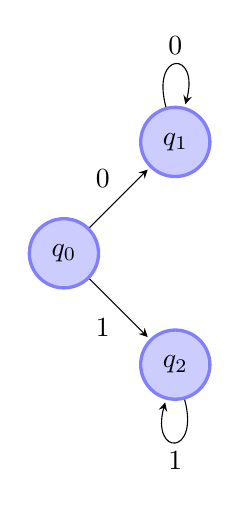
\begin{tikzpicture}[shorten >= 1pt, node distance=2cm, on grid, >=stealth,
every state/.style={draw=blue!50,very thick,fill=blue!20}]
\node[state]	(q_0)		{$q_0$};
\node[state]	(q_1) [above right=of q_0]	{$q_1$};
\node[state]	(q_2) [below right=of q_0]	{$q_2$};

\onslide<2>{\path[->]	(q_0)		edge				node	[above left]	{0}	(q_1);}
\only<1>{\path[->](q_0)	edge				node	[below left]	{1}	(q_2)
		(q_1)		edge	[loop above]	node				{0}	()
		(q_2)		edge	[loop below]	node				{1}	();}
\end{tikzpicture}
\end{frame}

% All of the following is optional and typically not needed. 
\appendix
\section<presentation>*{\appendixname}
\subsection<presentation>*{For Further Reading}

\begin{frame}[allowframebreaks]
  \frametitle<presentation>{For Further Reading}
    
  \begin{thebibliography}{10}
    
  \beamertemplatebookbibitems
  % Start with overview books.

  \bibitem{Author1990}
    A.~Author.
    \newblock {\em Handbook of Everything}.
    \newblock Some Press, 1990.
 
    
  \beamertemplatearticlebibitems
  % Followed by interesting articles. Keep the list short. 

  \bibitem{Someone2000}
    S.~Someone.
    \newblock On this and that.
    \newblock {\em Journal of This and That}, 2(1):50--100,
    2000.
  \end{thebibliography}
\end{frame}

\end{document}

